\documentclass[10pt]{article}


\usepackage{amssymb} %simbols
\usepackage[margin=0.92in]{geometry} %margins
\usepackage{graphicx} %for placing images


\usepackage{amsmath}
\usepackage[sc]{mathpazo} % Use the Palatino font
\usepackage[brazilian]{babel}
\usepackage[utf8]{inputenc}
\usepackage[T1]{fontenc} % Use 8-bit encoding that has 256 glyphs
\linespread{1.05} % Line spacing - Palatino needs more space between lines
\usepackage{microtype} % Slightly tweak font spacing for aesthetics


\usepackage{multicol} 
\usepackage{lettrine} % The lettrine is the first enlarged letter at the beginning of the text
\usepackage{titlesec} % Allows customization of titles
\renewcommand\thesection{\Roman{section}} % Roman numerals for the sections
\renewcommand\thesubsection{\Roman{subsection}} % Roman numerals for subsections
\titleformat{\section}[block]{\large\scshape\centering}{\thesection.}{1em}{} % Change the look of the section titles
\titleformat{\subsection}[block]{\large}{\thesubsection.}{1em}{} % Change the look of the section titles

\usepackage{fancyhdr} % Headers and footers
\pagestyle{fancy} % All pages have headers and footers
\fancyhead{} % Blank out the default header
\fancyfoot{} % Blank out the default footer
\fancyhead[C]{Projeto Final - Bancos de Dados $\bullet$ Dezembro 2013 $\bullet$ } % Custom header text
\fancyfoot[RO,LE]{\thepage} % Custom footer text



\begin{document}

\title{Taekwondo nos jogos olímpicos: modelo de banco de dados}% Article title
\date{}
\maketitle

\begin{center}
\author{Thomaz Macedo,  Eduardo Furtado\\Departmento de Ciência da Computação\\
Universidade de Brasília\\
Distrito Federal, Brasil\\
71009-000\\
tho.macedo@gmail.com, eduardoxfurtado@gmail.com
}
\end{center}

\begin{abstract}
\emph{O Brasil é a próxima sede das Olimpíadas, um enorme evento do qual pessoas mundo inteiro participam, direta ou indiretamente.  Um evento desse porte gera quantidade imensa de dados. Além de dados sobre as competições, informações úteis aos espectadores e turistas podem ser integradas ao contexto, gerando informações mais completas sobre a estruturação da cidade sede do evento. Como projeto, apresentamos, com o tema do esporte olímpico Taekwondo, um banco de dados pequeno para armazanar e gerenciar esses dados. O sistema foi integrado a uma  CRUD em  PHP sobre servidores servidores Apache, duas importantíssimas tecnologias relacionadas a bancos de dados web.  O banco de dados escolhido foi o MySQL e ferramentas como o SmartDraw e o MySQL Workbench foram utilizadas para o desenvolver o DER e o MER. O banco de dados foi instanciado em uma máquina servidor e uma VPN foi criada para permiir o acesso remoto}. \\ \\ \\
\end{abstract}

\begin{multicols}{2}

\section{Introdução}
Taekwondo é uma arte marcial de origem coreana praticada há mais de 50 anos e seu nome significa "o caminho dos pés e das mãos". As primeiras competições de nível mundial começaram a surgir em medos da década de 1970 mas apenas em 1988, nos jogos olímpicos de Seul, o Teakwondo foi introduzido no contexto de uma olímpiada. Participou nesse ano e em 1992 como esporte de demontração e em 2000, em Sidney, foi oficialmente integrado como esporte olímpico. Presente desde então em todas as edições, o Taekwondo é um dos esportes que mais gera medalhas: 8 no total. São quatro modalidades de peso para cada gênero de competidores. Um evento do porte de uma olimpíada requer um alto investimento em infra-estrutura por parte da cidade sede. Muitos parques esportivos devem ser reformados e adaptados, instalações devem ser construídas para receber os atletas e, além disso, toda a questão de mobilidade deve ser replanejada para atender ao grande número de turistas que vêm acompanhar o evento.  Em muitos casos é também necessário sinalizar toda a cidade,  preparar equipes de orientação ao turista e distribuir cartilhas e outros materiaisque possam auxiliar os não-locais em situações de emergência ou mesmo informar sobre restaurantes e hotéis mais próximos. Com o intuito de prover uma forma de disponibilizar e organizar os dados sobre as competições de Taekwondo nas olimpíadas e, ao mesmo tempo, agregar as informações úteis aos turistas, propomos nesse trabalho um banco de dados relacional que modela o contexto desse tipo de evento.

\section{Metodologia}
\subsection{DER - Diagrama Entidade Relacionamento}
O passo inicial do projeto foi a elaboração de  um DER onde as informações a respeito da competição possam ser vinculadas a informações úteis aos espectadores do evento e aos turistas. O local das competições é o elemento que permitiu associar todas essas informações. O desenho do projeto levou considerou o endereço geral como composto por cidade, bairro, endereço e descrição. O campo endereço no caso corresponde a o nome da rua, avenida ou quadra (considerando cidades como Brasília) e a descrição é que deve conter os detalhes como edifício, número, etc. Cada endereço está associado a um bairro que por sua vez se relaciona com  a cidade. É sabido que os jogos olímpicos têm sede em apenas uma cidade, mas considerando que o projeto possa ser utilizado para armazenar dados de mais de uma edição do evento, a existência de uma entidade cidade é justificada.\\ Pelo DER apresentado na Figura 1, percebe-se que pelo endereço da arena esportiva é possível vincular os hospitais e restaurantes mais próximos, assim como as linhas de ônibus que levam às proximidades do evento e essas informações podem ser então utilizadas ple a organização da competição para orientar os turistas. 

\end{multicols}

\begin{center}
\begin{figure}[h]
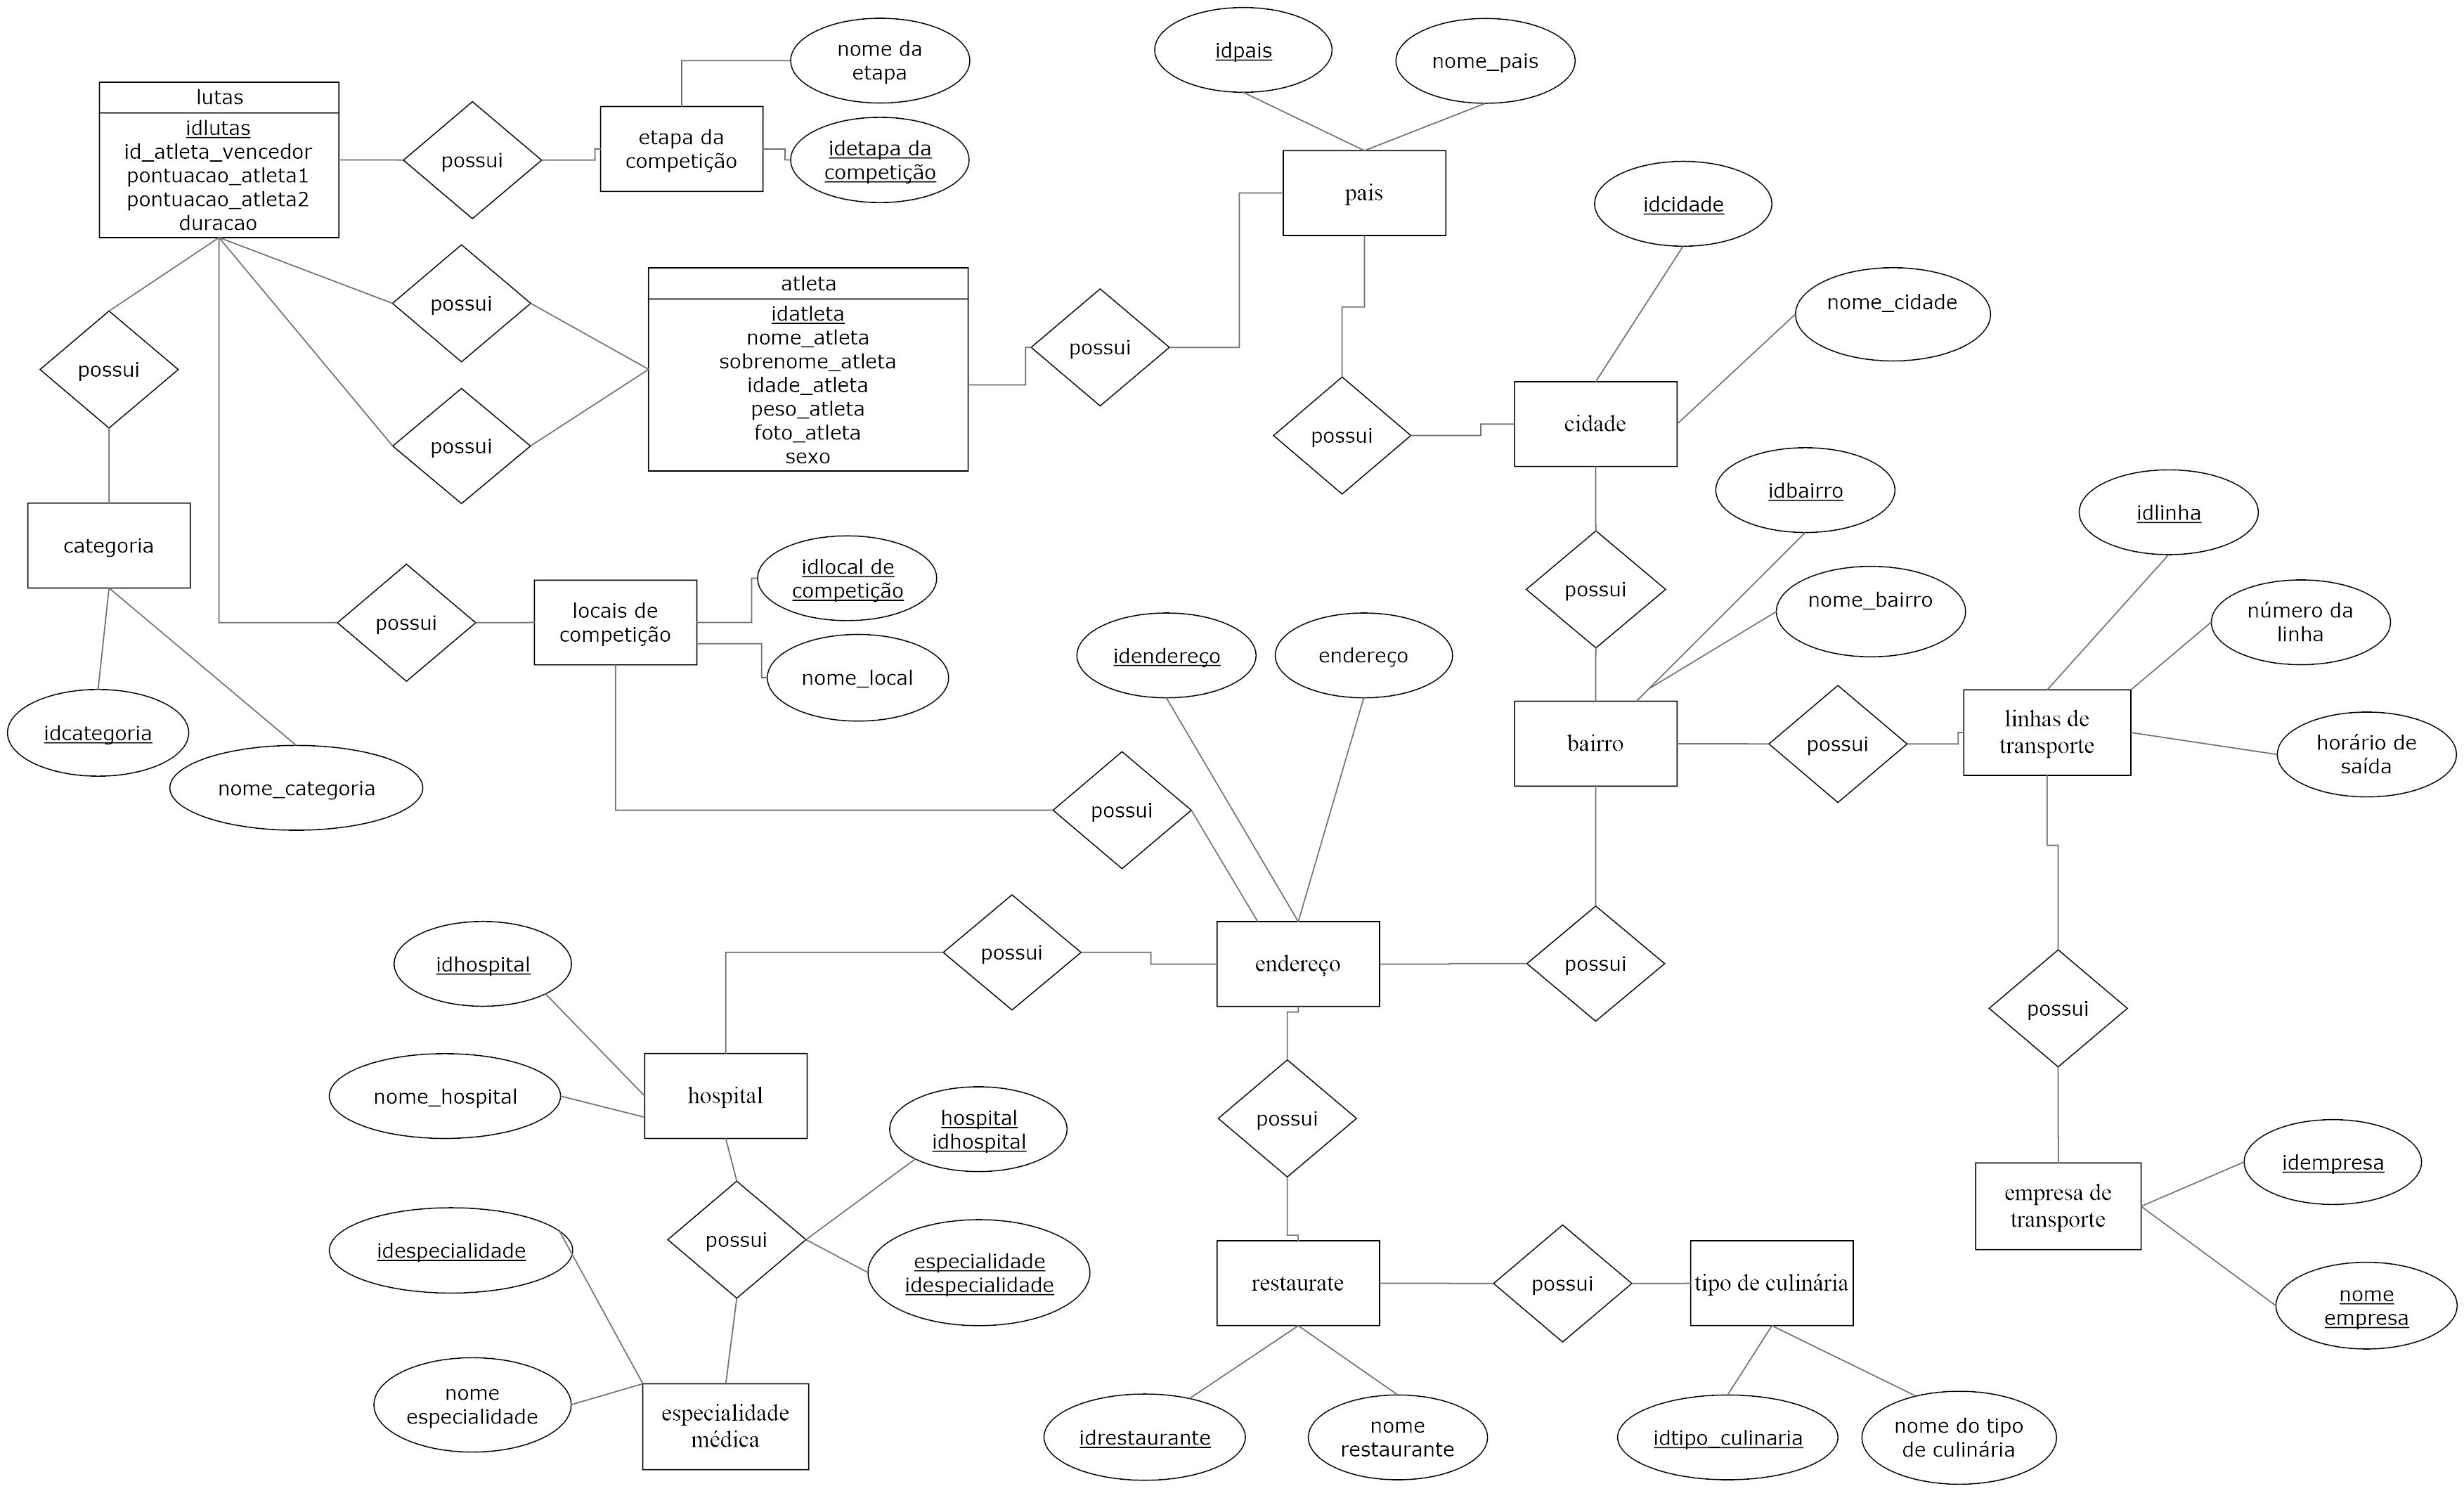
\includegraphics[scale=0.13]{der.jpg}
\caption{ Diagrama Entidade Relacionamento proposto}
\end{figure}
\end{center}

\begin{multicols}{2}
\subsection{MF - Modelo Físico}
O próximo passo é a escolha de um SGBD, para a implementação física do banco de dados. O grau de complexidade do projeto permite sua implementação em sistemas bem simples, como o SQLite, por exemplo. Porém, ao escolher um SGBD buscamos atender aos seguintes requisitos: opensource, gratuito, bem documentad e de ampla utilização em escala de produção. Justificadamente, foi esoclhido o MySQL 5 por apresentar todas as características mencioanadas anteriormente. O banco de dados escolhido foi obtido através do pacote Xampp 1.8.2, que traz Apache 2.4.7, MySQL 5.5.34 e PHP 5.4.22. Xampp tem sido utilizado em escala de produção em muitos sistemas web. \\
Após a instalação e configuração básica do pacote, foi necessária a instalação do MySQL Workbench 6.0 CE, o console de administração do MySQL. Trata-se de uma ferramenta bastante completa que traz todas as funcionalidades requeridas por um DBA e também possui funcionalidades de projetar um banco de dados a partir de modelos físicos. O modelo físico do banco foi gerado utilizando essa ferramenta e pode ser observado na Figura 2. É importante notar que o modelo físico traz, além dos relacionamentos descritos no DER, a referência explícita de chaves primárias e estrangeiras nas tabelas, pois o MF será utilizado para geraro script DDL de criação do banco e a referenciação correta entre as entidades é de extrema importância para uam implementação bem sucedida.

 \end{multicols} 

\begin{center}
\begin{figure}[h!]
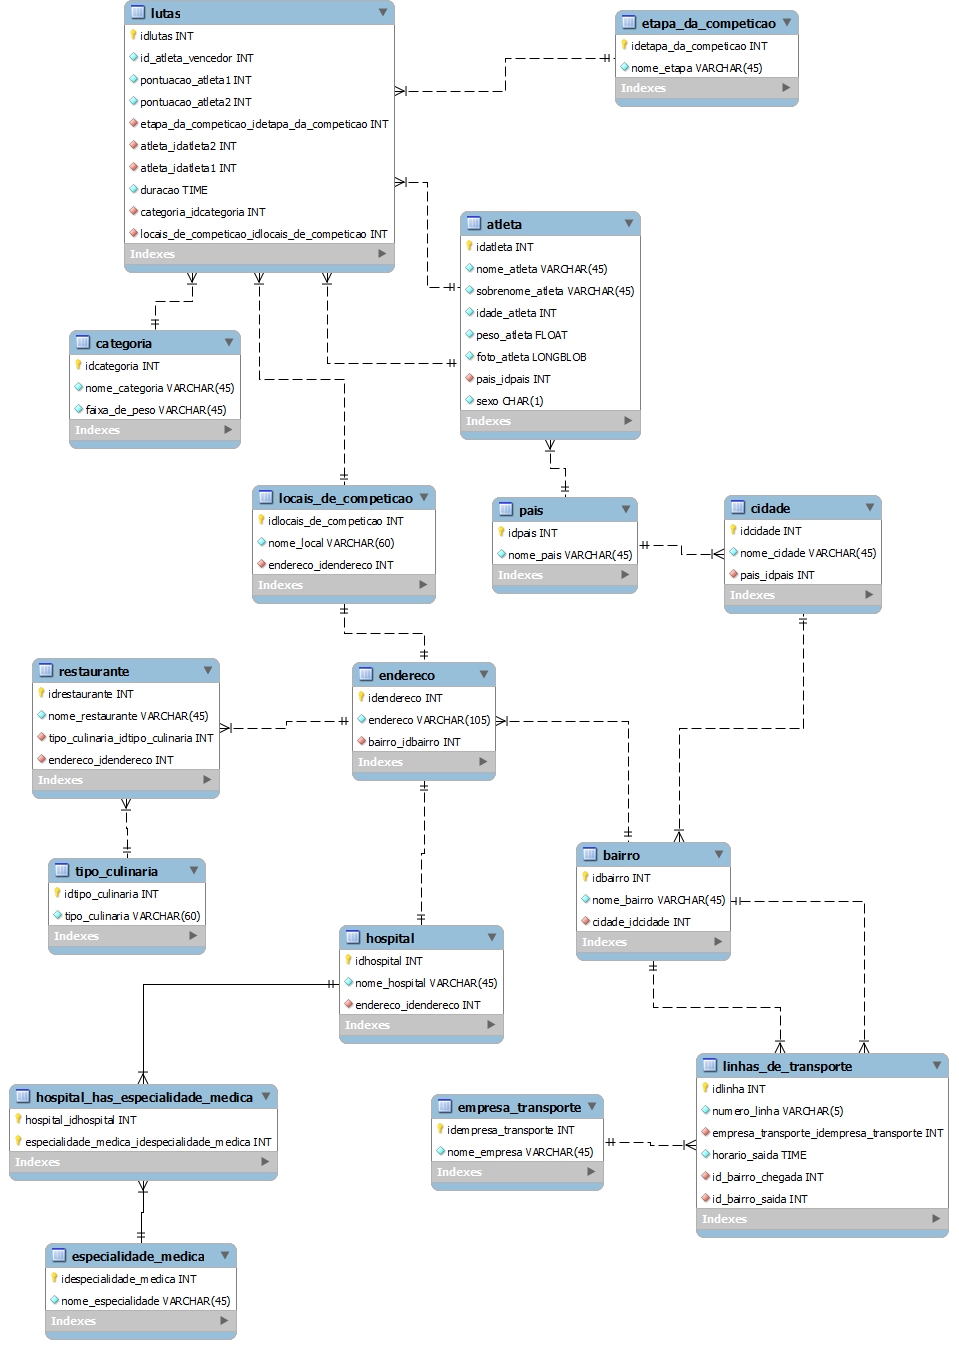
\includegraphics[scale=0.45]{mf.png}
\caption{Modelo físico do banco de dados}
\end{figure}
\end{center}

\begin{multicols}{2}
\subsection{Normalização}
Antes de executar o script de criação do banco a partir do modelo físico definido anteriormente, validou-se o modelo em realção à normalização das tabelas. A normalização de dados em um BD consiste numa série de procedimentos aplicados aplicados às tabelas que permitirão um armazenamento mais consistente e acesso mais eficiente ao dados. A normalização reduz a redundância em bancos de dados e reduz as chances de inconsistência. O trabalho original de Codd definiu 3 formas normais para bancos de dados relacionais (o conceito dessas formas normais não será abordado nesse artigo). É desejado que um banco de dados apresente tabelas na terceira forma normal, onde além de já estar na 2FN, todo atributo não chave da tabela não possuir dependência funcional transitiva em relação à chave primária. Diz-se que X $\rightarrow$ Y é uma dependência funcional transitiva na relação R se
existir um conjunto de atributos Z em R, que não sejam chave candidata de R, de tal forma que as dependências X $\rightarrow$ Z e Z $\rightarrow$ Y existem [1]. A tabela \emph{lutas} foi usada para verificar a normalização do modelo proposto.
\\ 
\emph{ lutas} (\underline{idlutas} , id\_atleta\_vencedor,  pontuacao\_atleta1,  pontuacao\_atleta2, etapa\_da\_competicao \_id\_etapa\_da\_competicao, id\_atleta2, id\_atleta1,  duracao, categoria\_id\_categoria, locais\_de\_competicao \_idlocais\_de\_competicao)
\\
A dependência funcional transitiva é dada pelos atributos \emph{  id\_atleta\_vencedor, etapa\_da\_competicao \_id\_etapa\_da\_competicao, id\_atleta2, id\_atleta1, categoria\_id\_categoria, locais\_de\_competicao \_idlocais\_de\_competicao}, que são referneciados pelas seguintes tabelas:
\\ 
\emph{atleta} (\underline{idatleta}, nome\_atleta, sobrenome\_atleta, idade\_atleta, idade\_atleta, peso\_atleta, foto\_atleta, pais\_idpais, sexo)
\\
pais\_idpais referencia pais(idpais)
\\ \\
\emph{categoria} (\underline{idacategoria}, nome\_categoria, faixa\_de\_peso)
\\ \\
\emph{locais\_de\_competicao} (\underline{idlocais\_de\_competicao}, nome\_local, endereco\_idendereco)
\\ endereco\_idendereco referencia endereco(idendereco)
\\ \\
Para todas as tabelas às quais atributos de \emph{lutas} faz referência, todos os atributos  são monovalorados, dependetes funcionais totais ou são referentes a outra tabela - onde a mesma estrutura se repete - o que faz com que todo o modelo, por fim, esteja na terceira forma normal.
\end{multicols}

\begin{multicols}{2}
\subsection{Álgebra Relacional}
Algumas informações informações importantes podem ser obtidas do modelo normalizado. Dentre as consultas mais comuns estão as que permitem conhecer os vencedores e da competição. Não há uma tabela que armazene diretamente esses dados, e portanto, informações desse tipo podem ser obtidas via consultas ao banco. Para exemplificar, o campeão da categoria Peso Mosca Masculino a seguinte consulta deve ser realizada:
\\
 \emph{$\Pi$nome\_atleta ($\sigma$ id\_atleta\_vencedor = idatleta $\bigwedge$  ($\sigma$ etapa\_da\_competicao\_idetapa\_da\_competicao = idetapada\_da\_competicao $\bigwedge$ idetapa\_da\_competicao = 'Final' ) $\bigwedge$ ($\sigma$ categoria\_idcategoria = idcategoria $\bigwedge$ nome\_categoria =' Peso Mosca Masculino' (lutas X categoria )) (lutas X atleta))}
\\ \\
Do mesmo modo, podemos usar a mesma consulta para verificar a terceira colocada da categoria Peso Pesado Feminino: 
\\
 \emph{$\Pi$nome\_atleta ($\sigma$ id\_atleta\_vencedor = idatleta $\bigwedge$ ($\sigma$ etada\_da\_competicao\_idetapa\_da\_competicao = idetapada\_da\_competicao $\bigwedge$ idetapa\_da\_competicao = 'Semifinall' ) $\bigwedge$ ($\sigma$ categoria\_idcategoria = idcategoria $\bigwedge$ nome\_categoria =' Peso Pesado Feminino' (lutas X categoria )) (lutas X atleta))}
\\ \\
 A informação dos hospitais mais próximos ao local de competição pode ser obtida pela seguinte consulta:
\\ 
\emph{ $\Pi$nome\_hospital  ($\sigma$  bairro= id\_bairro ($\sigma$ endereco\_idendereco = idendereco (hospital X endereco) $\bigwedge$ endereco\_id\_endereço = id\_endereco (locais\_de\_competicao X endereco)) (endereco X bairro))} 

\subsection{CRUD}
 CRUD é o termo utilizado em computação para descrever as quatro operações básicas relacionadas à persistêcnia no contenxto de bancos de dados: Create, Read, Update e Delete. Na maior parte dos cados, CRUDs são implementadas  através de uma aplicação que capaz de se comunicar e prover uma interface gráfica que permite ao usuário realizar suas operações sem conhecer o esquema do bando e sem escrever querys SQL. O PHP foi escolhido como linguagem para desenvolvimetno da CRUD por já constar no pacote Xampp e por ser voltada para a web. É muito utilizada para construir aplicações sobre MySQL e com documentação extensa na web. Muitos códigos de exemplo podem ser facilmente encontrados e adaptados para casos de uso amis específicos. A interface desenvolvida foi baseada numa antiga aplicação de um dos integrantes do projeto. \\
\\Como alternativa para o CRUD desenvolvido em PHP, há um software mais robusto, completo e amplamente utilizado no mercado, o \emph{phpMyAdmin}, que é um sistema completo para gerenciar bancos de dados, mas que também  pode ser utilizado como uma CRUD, mediante a criação de um usuário com permissões restritas a apenas estas operações básicas no banco de dados, que pode acessar o sistema do phpMyAdmin para tal.

\end{multicols}

\begin{center}
\begin{figure}[h!]
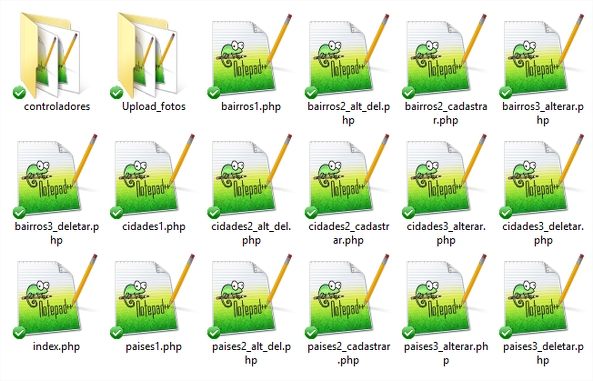
\includegraphics[scale=0.45]{crud.jpg}
\caption{Estrutura do CRUD desenvolvido em PHP}
\end{figure}
\end{center}


\begin{center}
\begin{figure}[h!]
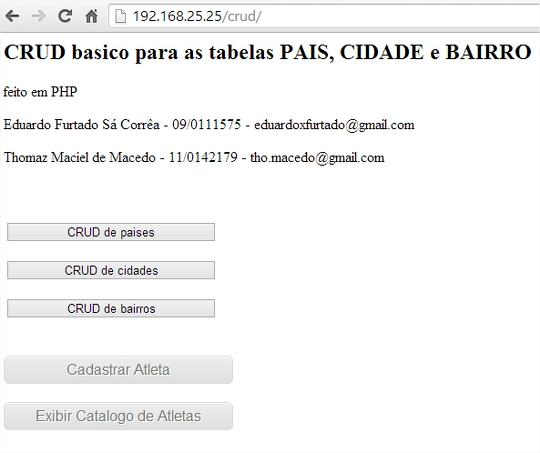
\includegraphics[scale=0.5]{crud1.jpg}
\caption{CRUD - Tela inicial da aplicação}
\end{figure}
\end{center}


\begin{center}
\begin{figure}[h!]
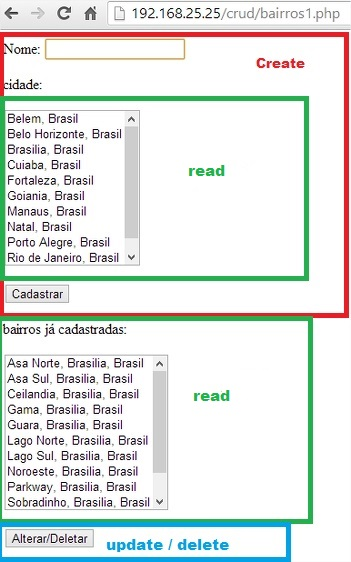
\includegraphics[scale=0.7]{crud2-bairros.jpg}
\caption{CRUD - exemplo}
\end{figure}
\end{center}


\begin{center}
\begin{figure}[h!]
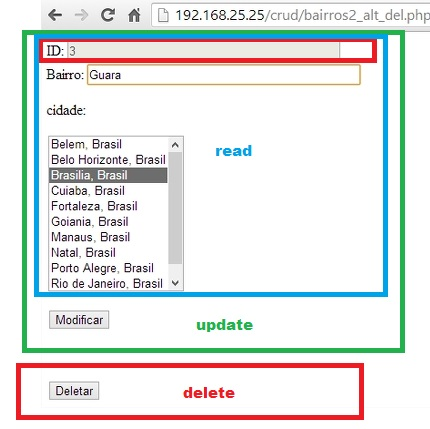
\includegraphics[scale=0.8]{crud3-bairros-altdel.jpg}
\caption{CRUD - Outro exemplo}
\end{figure}
\end{center}

\begin{center}
\begin{figure}[h!]
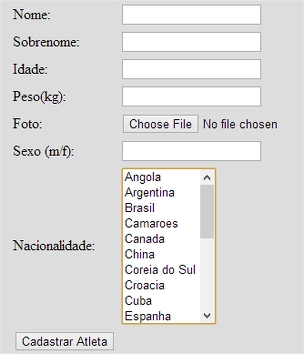
\includegraphics[scale=0.7]{crud5-atletas.jpg}
\caption{CRUD - Exemplo do cadastro de atletas com fotos}
\end{figure}
\end{center}

\begin{center}
\begin{figure}[h!]
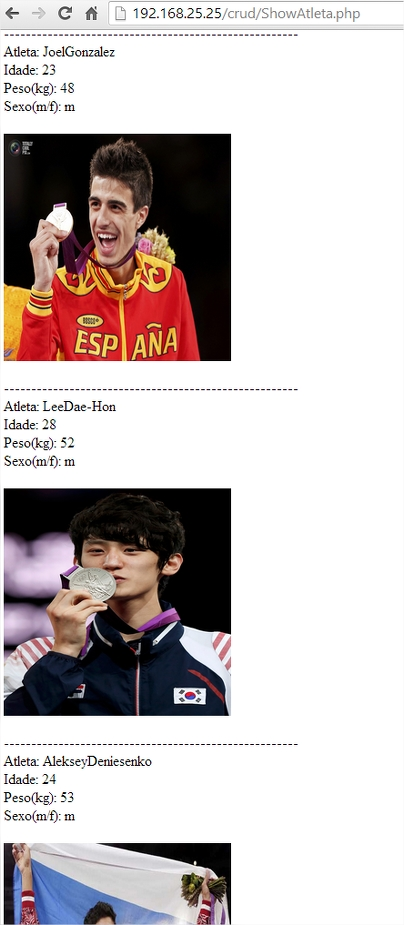
\includegraphics[scale=0.35]{crud7-atletas.jpg}
\caption{CRUD - Módulo de exibição das entradas cadastradas na tabela atletas}
\end{figure}
\end{center}


\begin{center}
\begin{figure}[h!]
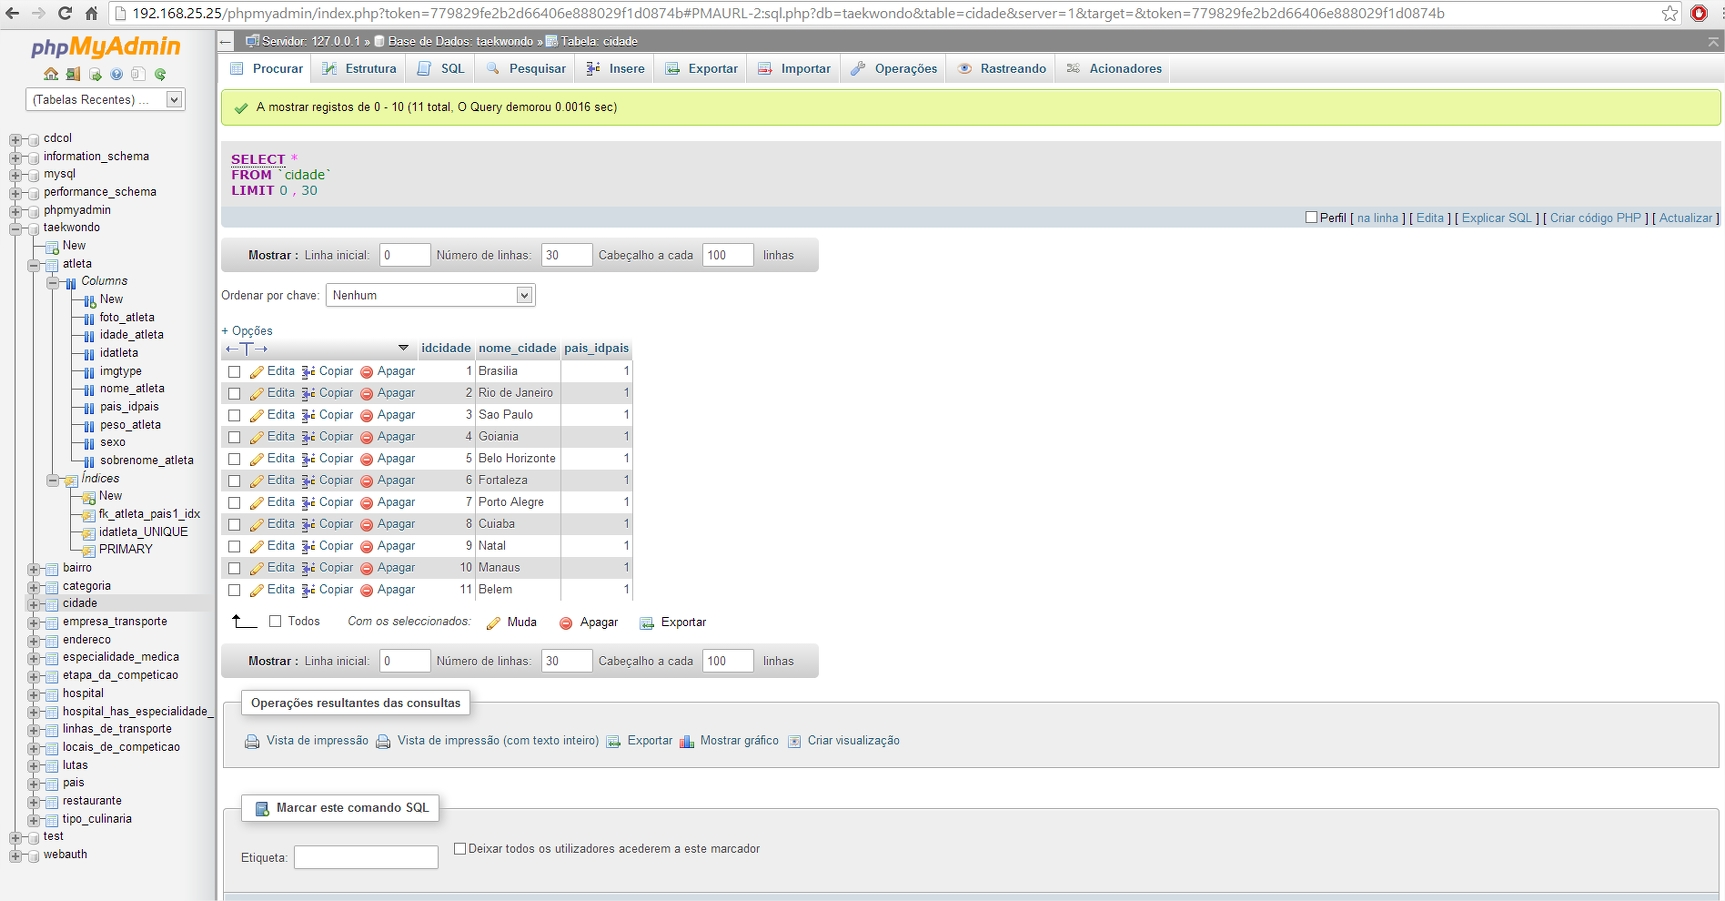
\includegraphics[scale=0.25]{phpmyadmin.jpg}
\caption{Ferramenta phpmyadmin}
\end{figure}
\end{center}

\begin{multicols}{2}


Muitos dos dados do banco foram povoados utilziando a própria aplicação CRUD desenvolvida, outros foram adicionados com queries escritas pelos integrantes e ainda outros foram adicionados utilizando a ferramenta phpmyadmin.
\\Os resultados são satisfatórios, e consistem de um banco funcional e populado. 

\section{Resultados}
O banco de dados criado para o projeto é capaz de gerenciar dados referentes à competição de taekwondo, dispondo de dados sobre as lutas como pontuação de cada atleta, data de realização e local de realização e relacionar essas informações com outras úteis apra turistas e espectadores através da chave identificadora \emph{idbairro} da tabela \emph{bairro}. A CRUD, embora não cutomizada, atende aos requisitos mínimos para uma aplicação que recebe essa nomenclatura e pode ser adaptada para atender às demais tabelas do modelo, não só as 3 testadas nesse projeto. \\ O modelo proposto é capaz de atender a várias edições do evento, já que possui uma tabela \emph{cidade} e essa pode ser referenciada pelos locais de competição (indiretamente). O projeto não só abordou aspectos relacionados a banco de dados relacionais como também aborda o paradigma de bancos de dados web, visto que todas as ferramentas do pacote Xampp foram utilizadas e a VPN arquitetada para o projeto confere as propriedades de Web DB ao sistema, através das máquinas conectadas a essa rede. O projeto foi bem sucedido e atende a todas a todos os requisitos da especificação.

\begin{thebibliography}{9}

\bibitem{site1}
  http://support.microsoft.com/kb/283878/pt-br
  \emph{Descrição dos conceitos básicos de normalização de banco de dados}\\
Acessado: 10/12/2013

\bibitem{site2}
http://www.youtube.com/watch?v=JhWVi-pY43Q
  \emph{Tutorial on Storing and Retriving images along with text from mysql database}\\
Acessado: 08/12/2013

\bibitem{site3}
http://www.wikinewsfacts.com/php-scripts-codes-examples/php-crud-example-1
  \emph{PHP. MYSQL. CRUD example: Create Retrieve Update Delete}\\
Acessado: 09/12/2013

\bibitem{site3}
Elmasri, R.; Navathe \\
\emph{Fundamentals of Database Systems,}
 Sixth Edition, Pearson, 2010, \\
pag 161-179




\end{thebibliography}

\end{multicols}


\end{document}
